Voici ci-dessous, la structure originale de la machine au commencement de ce projet de Bachelor :
\begin{figure}[H]
  \centering
  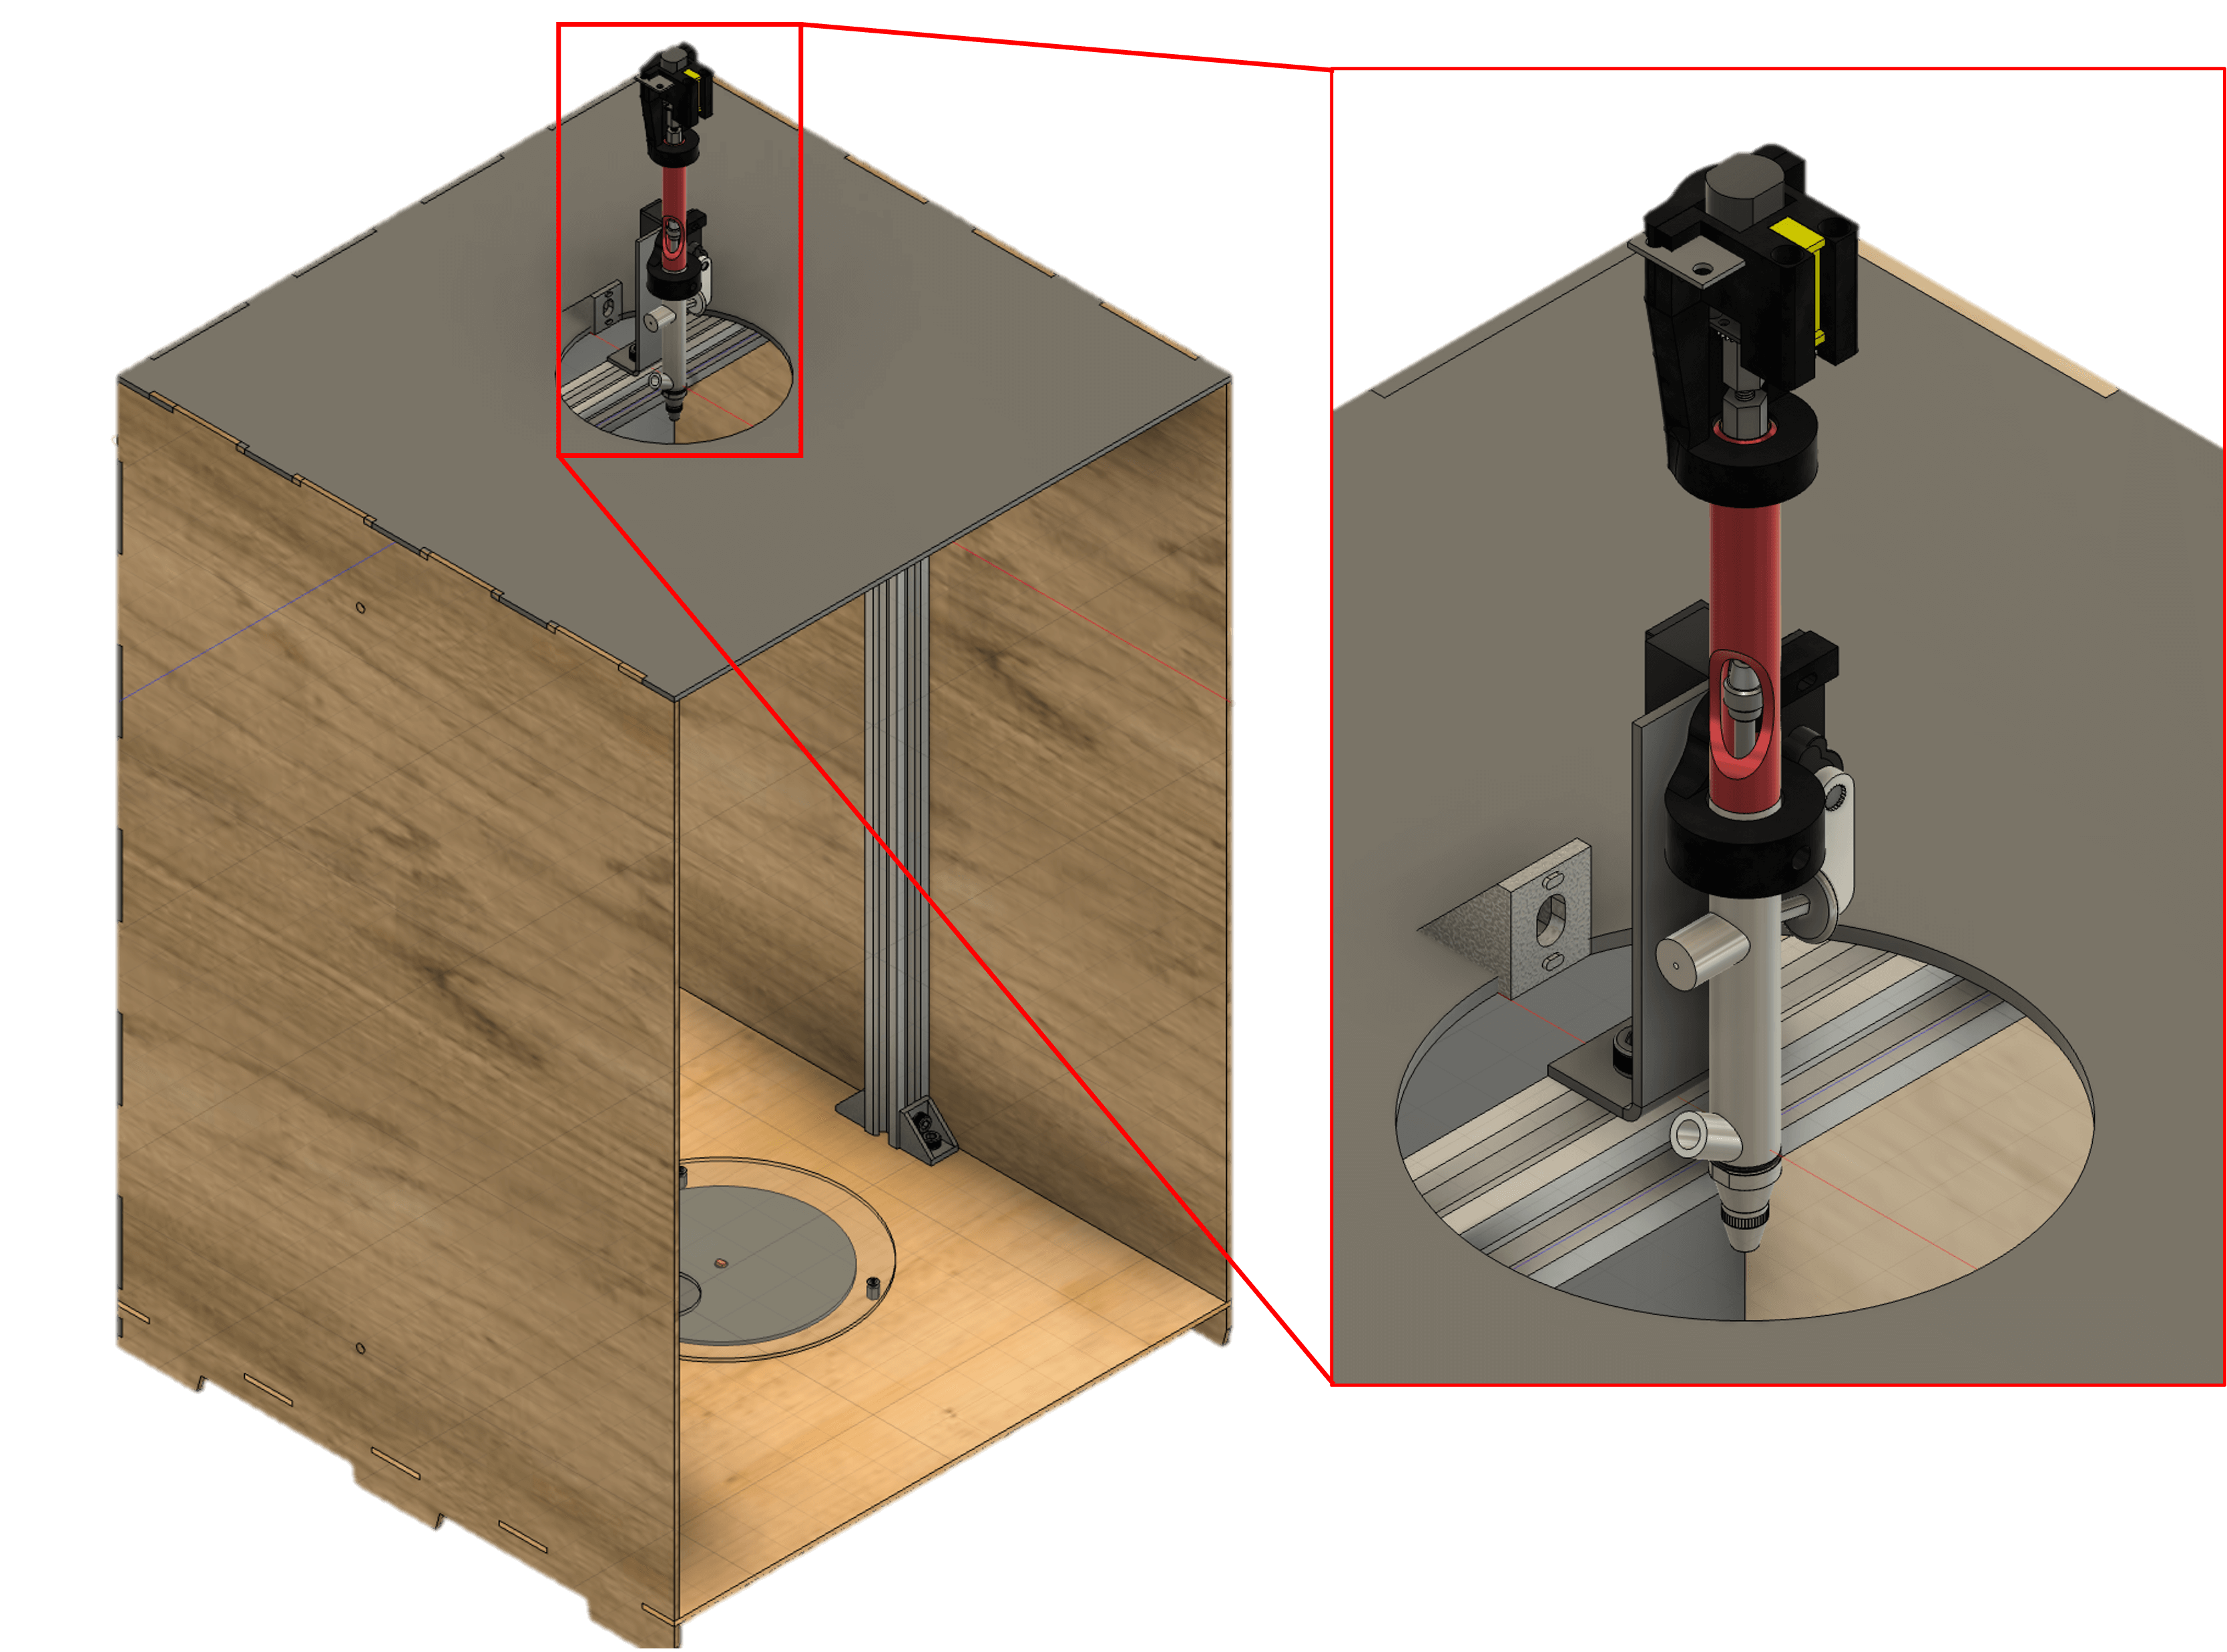
\includegraphics[width = \textwidth]{assets/figures/situation_initiale/machine_initiale.png}
  \caption[Machine originelle]{Machine originelle, avec un zoom sur le système de projection}
  \label{fig:Machine_originale}
\end{figure}

\newpage
La machine de projection se basait sur un aérographe robotisé, où des moteurs géraient les parties mobiles
de l'aérographe qui seraient normalement actionnée à la main :
\begin{figure}[H]
  \centering
  \begin{subfigure}{.35\textwidth}
    \centering
    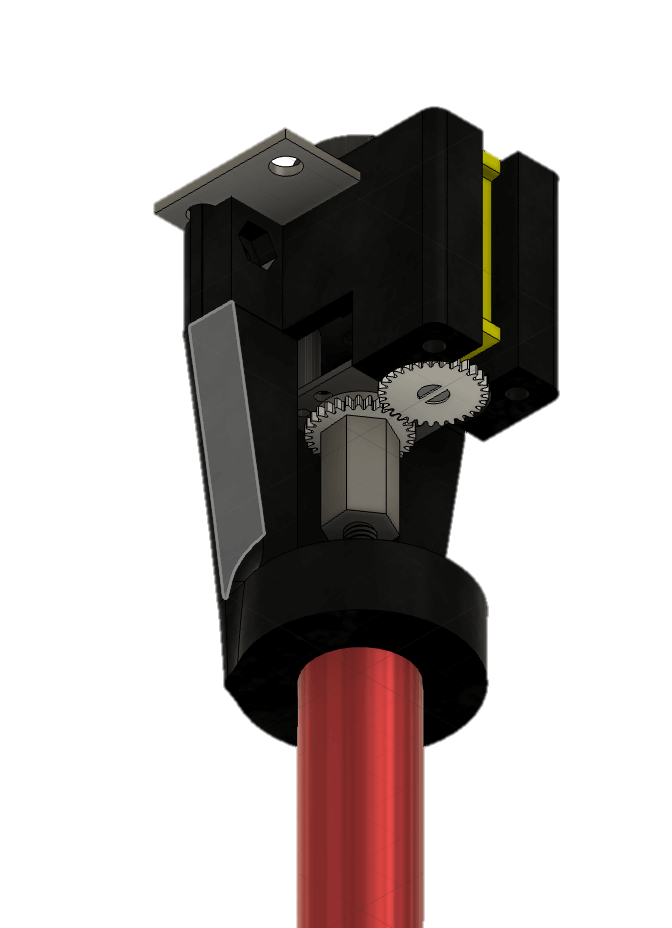
\includegraphics[width=1\linewidth]{assets/figures/situation_initiale/robotisation_aiguille.png}
    \caption{Robotisation de la position de l'aiguille}
    \label{fig:robot_aiguille}
  \end{subfigure}%
  \begin{subfigure}{.65\textwidth}
    \centering
    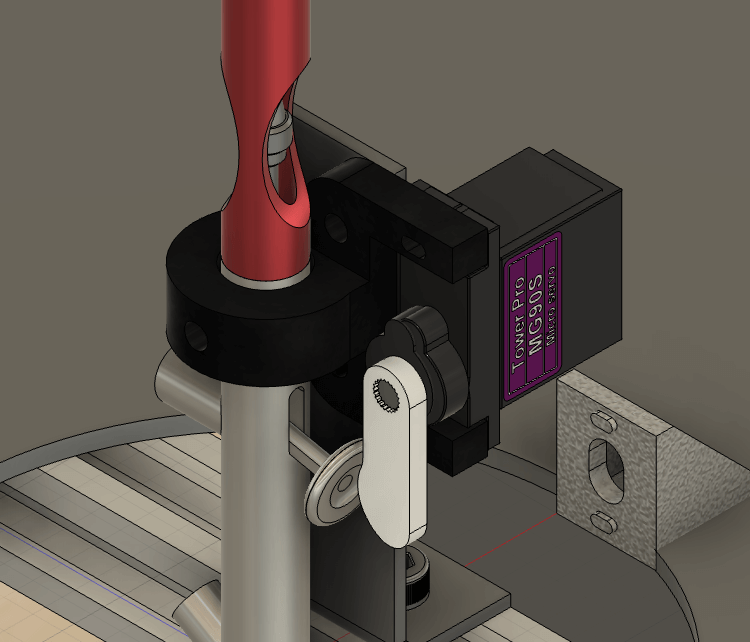
\includegraphics[width=.75\linewidth]{assets/figures/situation_initiale/Robotisation_projection.png}
    \caption{Robotisation du button d'activation du spray}
    \label{fig:robot_spray}
  \end{subfigure}
  \caption{Différentes robotisations de la machine originale}
  \label{fig:robotisations_aerographe}
\end{figure}

Un moteur pas-à-pas de type \textbf{28byj-48}, est situé en bas de l'appareil, ce dernier sert à faire tourner l'écran sur lui même,
c'est donc aussi où l'écran sera disposé lors de sa fabrication:
\begin{figure}[H]
  \centering
  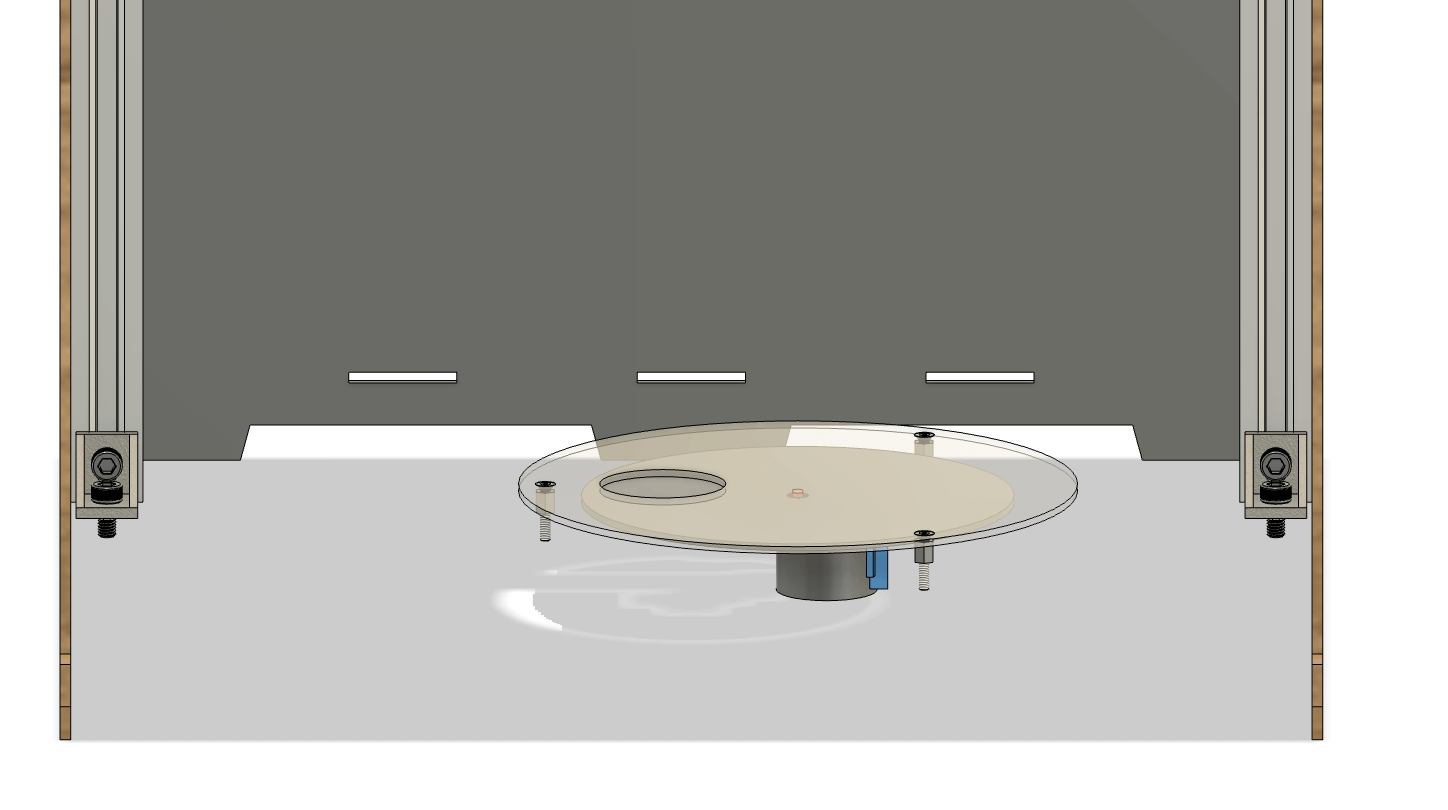
\includegraphics[width = \textwidth]{assets/figures/situation_initiale/rotation_ecran_initiale.png}
  \caption[Rotation écran initiale]{Système de rotation de l'écran}

\end{figure}

\newpage
Tout ces éléments sont contrôlés par un PCB et un arduino nano :
\begin{figure}[H]
  \centering
  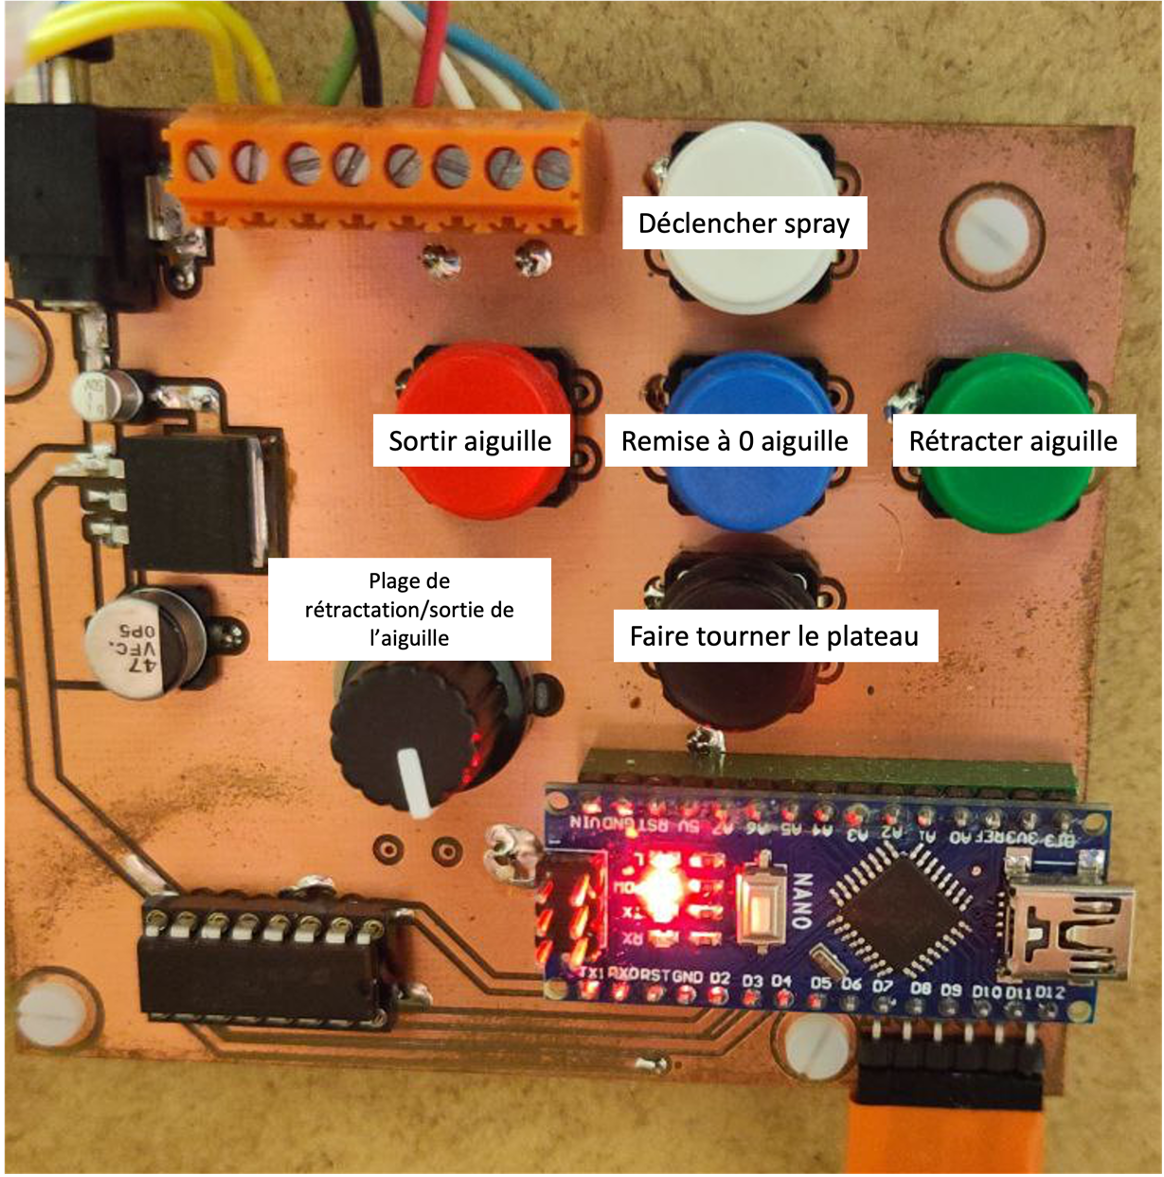
\includegraphics[width = 0.8\textwidth]{assets/figures/situation_initiale/PCB_machine_originale.png}
  \caption[PCB machine initiale]{PCB de la machine initiale et légende de chaque boutons}\label{PCB_machine_initial}
\end{figure}

\newpage
\section{Problèmes avec la machine}
En effet, la machine d'origine présente plusieurs inconvénients.
\subsection{Aérographe}
\subsubsection{Motorisation}
Comme montré dans la \autoref{fig:robotisations_aerographe}, l'aérographe est robotisé avec un moteur DC pour contrôler l'aiguille et un servo moteur pour activer
ou désactiver la projection de liquide. Ces deux éléments sont capricieux, le moteur DC de l'aiguille est relié à un encodeur (pour calculer la position de l'aiguille) à l'aide de deux petits engrenages en
plastique, ces engrenages en plastiques étant tout petits ils se sont usés, en plus de cela l'encodeur est monté seulement par compression sur le support du moteur, donc au fil des utilisations, les efforts
normaux des engrenages repoussent l'encodeur, le moteur ne sait donc plus où il se trouve et se met à tourner indéfiniment.

De plus la pièce qui tient le moteur et qui se fixe sur l'aérographe n'exerce pas assez de pression sur ce dernier, si l'aiguille résiste lors de son mouvement
la pièce de support se délogera de son emplacement :

\begin{figure}[H]
  \centering
  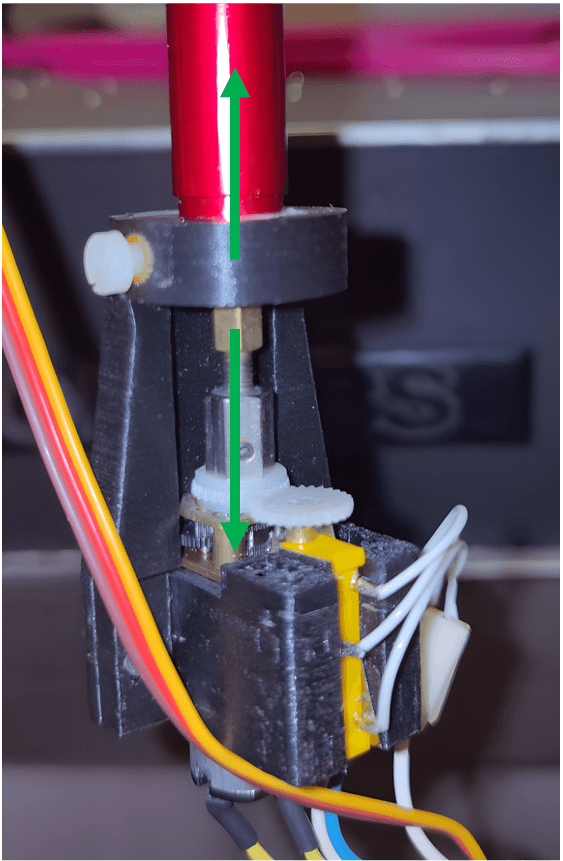
\includegraphics[width = 0.5\textwidth]{assets/figures/situation_initiale/moteur_desolidarisation_aerographe.png}
  \caption{Support moteur désolidarisé}
\end{figure}


\newpage
\subsubsection{État général}
Concernant l'état général de l'aérographe, ce dernier n'est pas idéal.
Le joint de la tête de projection est en bout de vie, il fuit et fait des bulles lors de l'utilisation de la machine:
\begin{figure}[H]
  \centering
  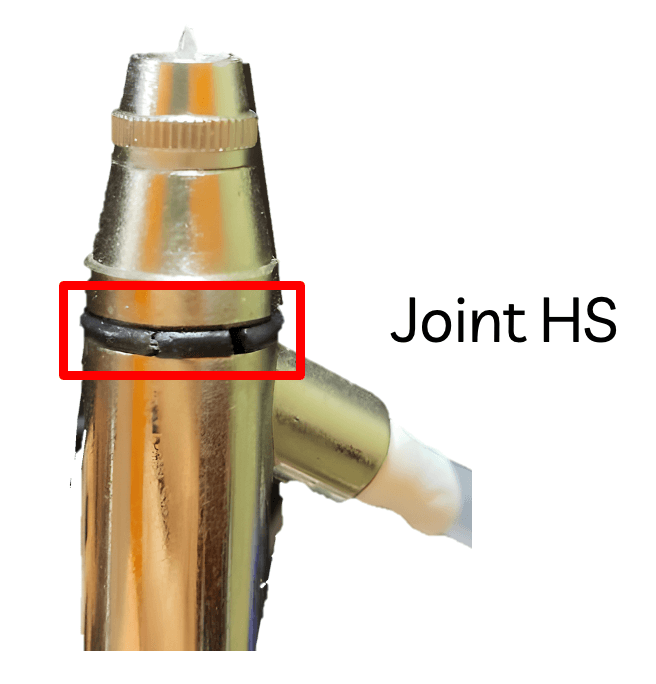
\includegraphics[width = 0.5\textwidth]{assets/figures/situation_initiale/joint_aerographe_HS.png}
  \caption{Joint sec et craquelé}
\end{figure}

Le support de l'aérographe qui permet de maintenir ce dernier sur le profilé alu du caisson de la machine est craqué,
ce dernier ne remplis plus sa fonction, l'aérographe bouge dans tout les sens et tourne sur lui-même :
\begin{figure}[H]
  \centering
  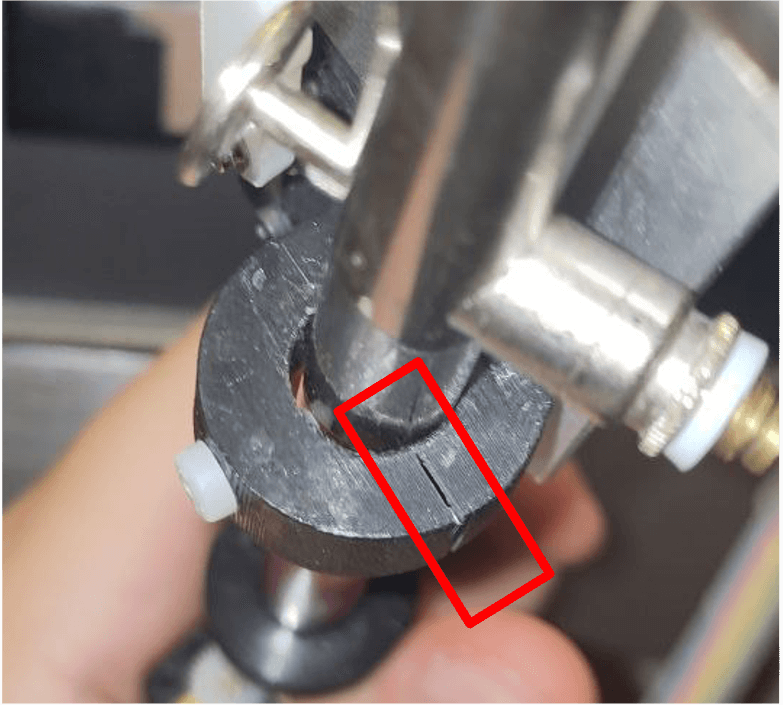
\includegraphics[width = 0.5\textwidth]{assets/figures/situation_initiale/support_aerographe_casse.png}
  \caption{Support aérographe cassé}
\end{figure}
En plus de cela, l'aérographe n'est pas conçu pour fonctionner avec un réservoir de liquude externe, il a fallu adapter ce dernier avec un tube plastique.
Il faut aussi savoir que raccorder l'aérographe au système d'air comprimé de l'école n'est pas possible sans une multitudes d'adaptateurs, il a donc fallu emprunter
un compresseur à l'atelier mécanique.

\newpage
\subsection{Interface utilisateur}
Pour contrôler la machine, un circuit imprimé est apposé sur son flanc (c.f \autoref{PCB_machine_initial}).
À noter que les fonctions des boutons décritent ci-dessus sont hypothétiques, nous n'avons pas pu retrouver le code
source du microprocesseur pour comprendre plus précisemment les actions de chaques boutons. Il est intéressant de remarquer
que les fonctions sont bloquantes, si on déclanche le spray, la fonction de spray doit être terminée, ce qui pose certains problèmes :

\begin{itemize}
  \item Si le capteur de position de l'aiguille est défaillant, le programme reste coincé.
  \item La fonction "faire tourner le plateau" est inutile car non exécutable lors de la fabrication de l'écran
\end{itemize}

\subsection{Fonctionnement}

Tout les éléments cités précédemment rendent la fabrication d'écrans fastidieuse, surtout si l'objectif est de manipuler précisemment les paramètres de fabrication.
Venant s'ajouter à ceci, l'utilisation de l'aérographe à la vertical pose un problème de taille, ce dernier fait des grosses gouttes qui tombent inévitablement sur
les écrans de phases. Pour contourner ce problème et se familiariser avec la fabrication d'écrans, il été déterminé que retourner la machine pour contrer les gouttes
soit la meilleure solution avant le dévoleppement de la solution décrite plus tard dans ce rapport.

\begin{figure}[H]
  \centering
  \includegraphics[width = 1\textwidth]{assets/figures/situation_initiale/machine_retournée.png}
  \caption{Nouvelle orientation de la machine}
\end{figure}

\newpage
\section{Fabrication des écrans}
Pour fabriquer les écrans, un mélange de vernis d'acrylique transparent brillant soluble dans l'eau(choix expliqué dans \color{red}INSéRER REF éTAT DE L'ART\color{black}) et d'eau (4 part d'eau pour une part d'acrylique),
c'est un des mélanges utilisés par la personne ayant développé le système d'origine, c'est un mélange assez liquide facile à projeter.

\begin{figure}[H]
  \centering
  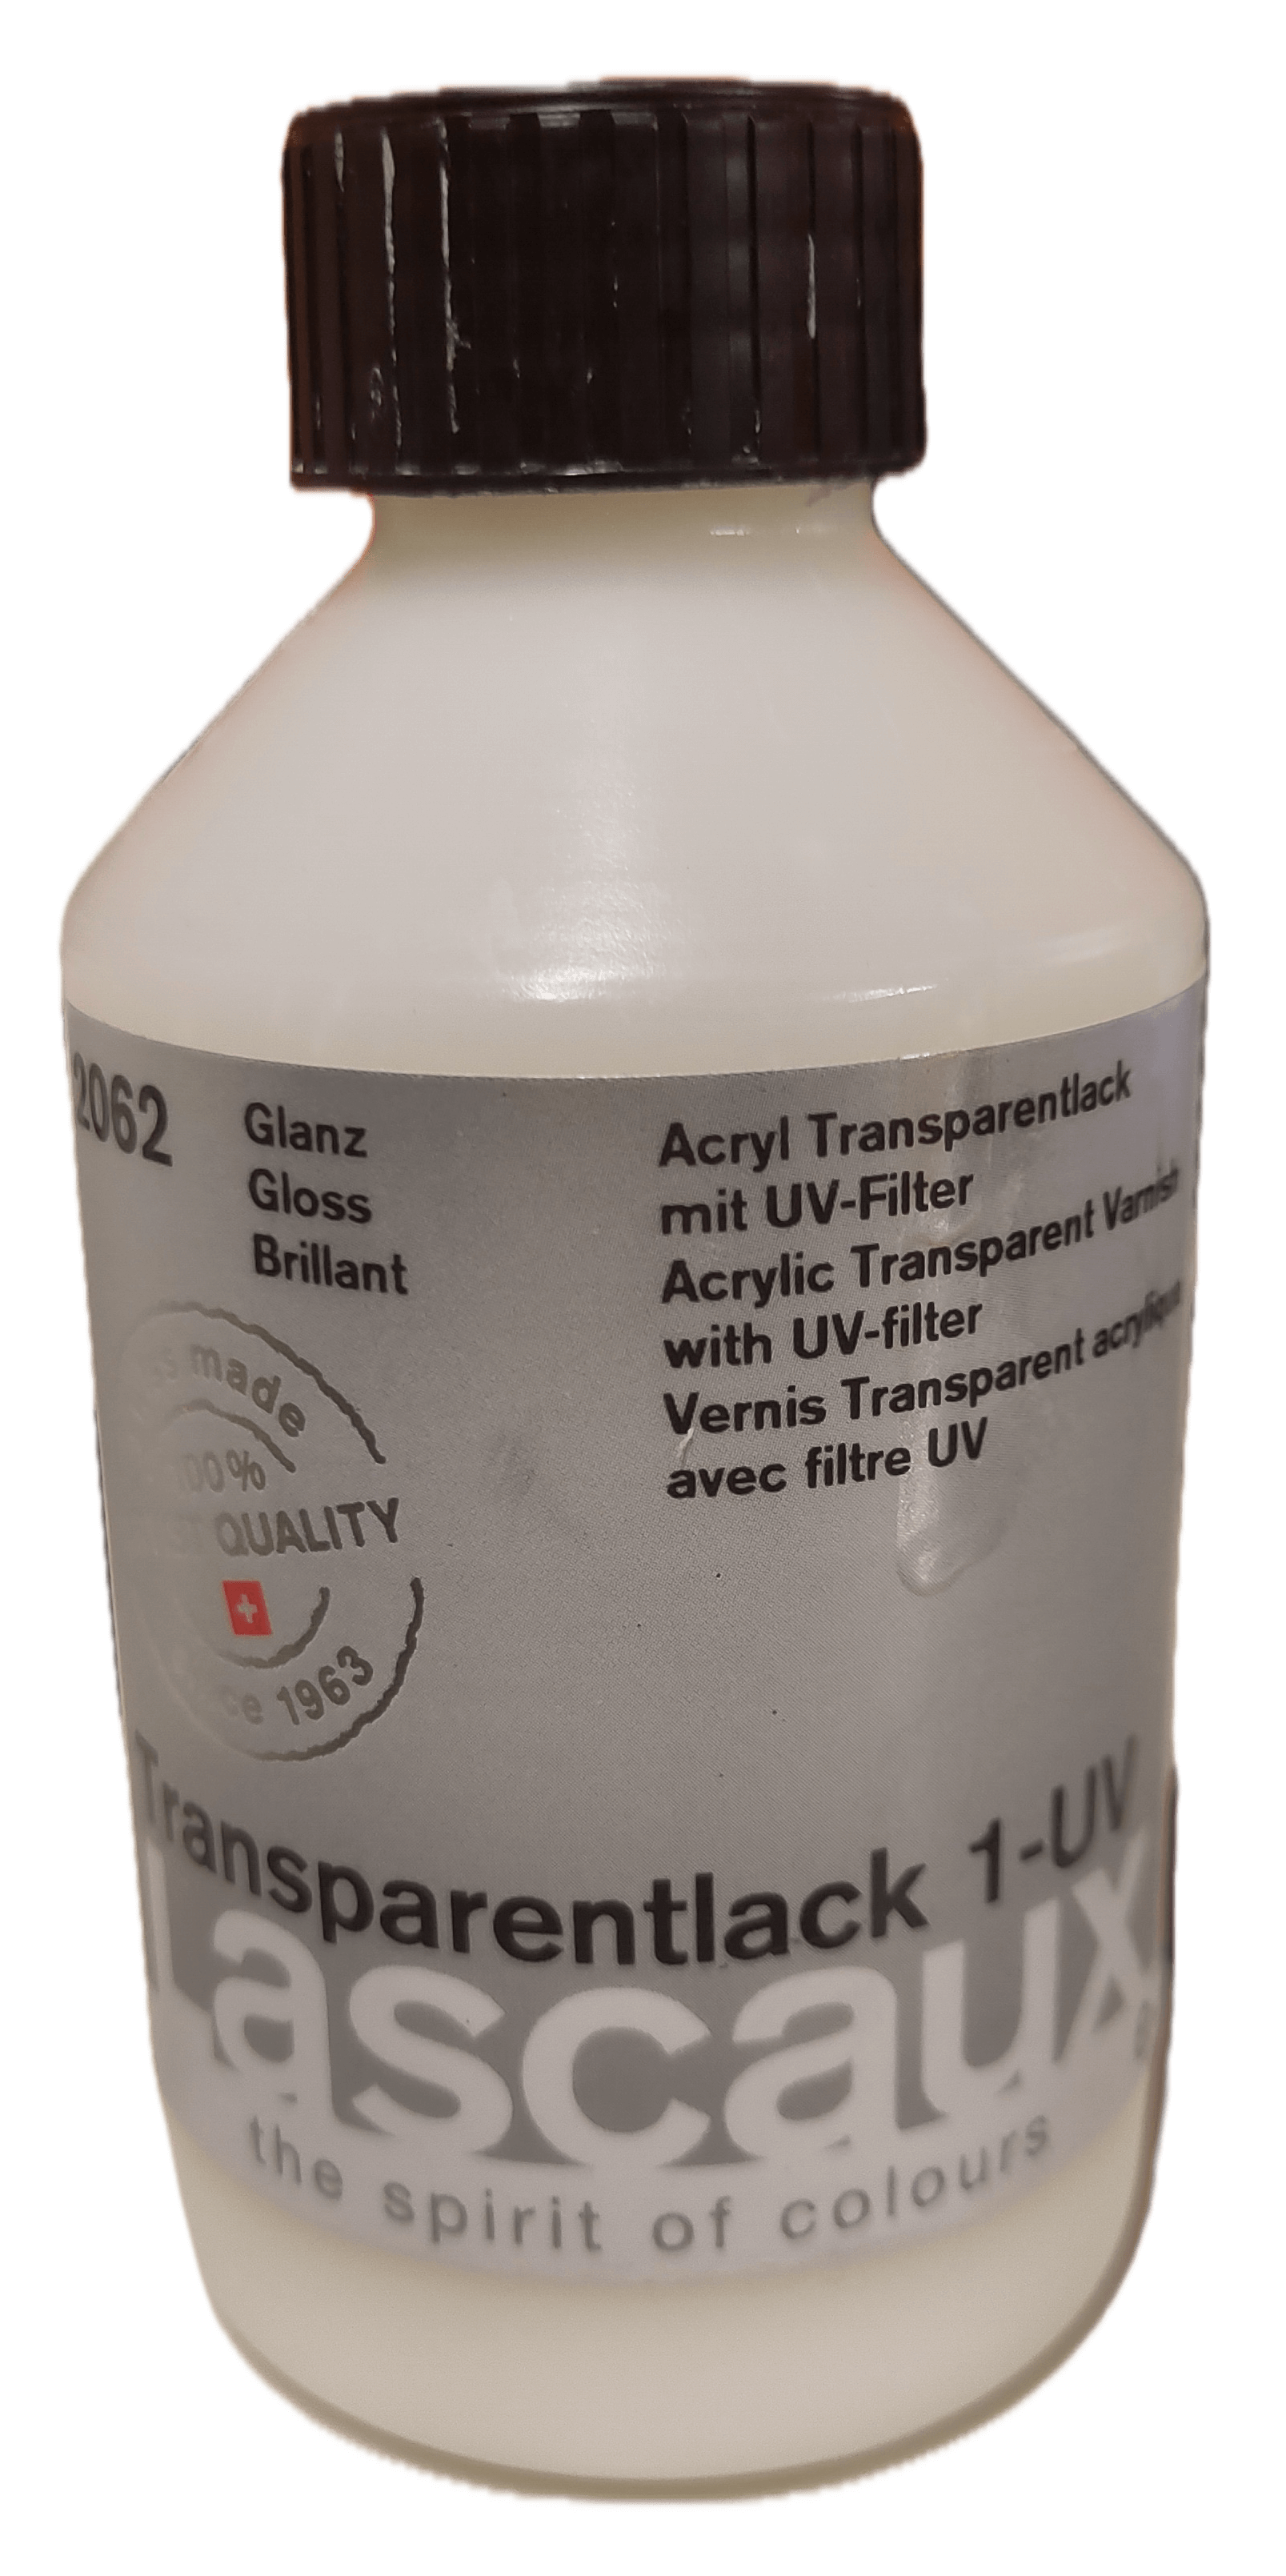
\includegraphics[width = 0.25\textwidth]{assets/figures/situation_initiale/Lascaux_vernis_brillant.png}
  \caption{Vernis brillant de la marque Lascaux}
\end{figure}

À ce stade du projet, il a été déterminé que la plage d'exposition aux goutte idéale pour fabriquer un écran de turbulences se situait entre 15 et 20 secondes sur l'ancienne machine.\footnotemark
Ayant donc pour résultat l'écran suivant :
\begin{figure}[H]
  \centering
  \includegraphics[width = 0.6\textwidth]{assets/figures/situation_initiale/écran_phase_beta.png}
  \caption{Écran de phase considéré comme bon}\label{fig:ecran_phase_beta}
\end{figure}

\footnotetext{Note personnelle : Cette hypothèse vient du fait d'une incompréhension de ma part, en effet, j'avais compris que l'écran de turbulences se composait d'une surface pas complétement recouverte de vernis, mais plus de goutelette
  isolées (mais rapprochées) formant de petites lentilles. Cette hypothèse fut invalidée après discussion avec M. Jolissaint.}

\newpage

En observant au microscope l'écran de la \autoref{fig:ecran_phase_beta}, on obtient l'image suivante :

\begin{figure}[H]
  \centering
  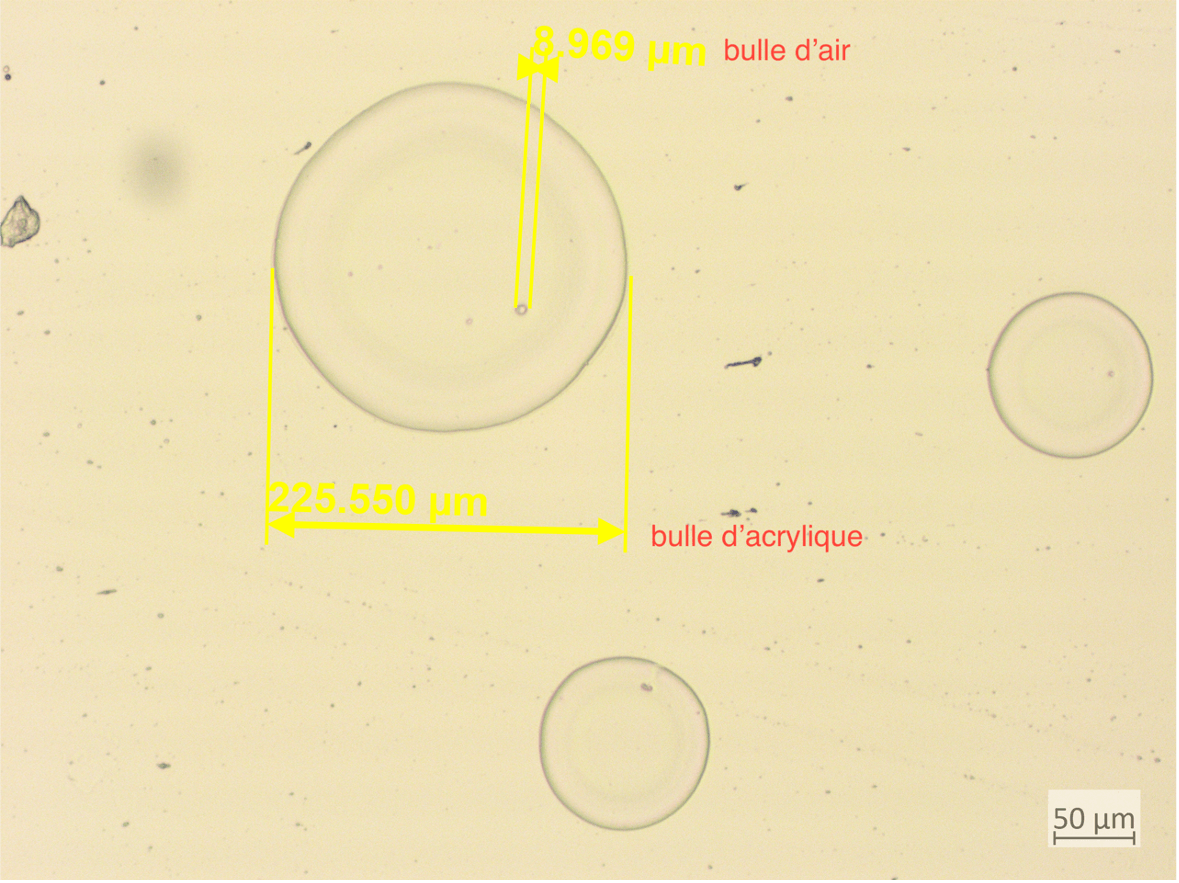
\includegraphics[width = 0.9\textwidth]{assets/figures/situation_initiale/observation_microscope.png}
  \caption{Observation d'un écran de phase au microscope}\label{fig:ecran_phase_beta_microscope}
\end{figure}
Il est donc possible d'observer la taille des goutelettes d'acrylique, et de constater que ces dernières contiennent des bulles d'air microscopiques.
On peut aussi observer l'espace entre chaques goutelettes ($250\pm 50 \mu m$).

Comme dit précédemment ces écrans ont été considérés comme bons à tort, en effet, il faudrait une couche complète d'acrylique sur le plastique, et donc pas une structure sous forme de goutelettes espacées.
Il sera toutefois intéressant de caractériser les écrans produits par cette première technique avec le programme développé lors de ce projet (c.f \color{red} AJOUTER REF à ANALYSE \color{black}).

\section{Conclusion}
Pour conclure cette section qui a constitué les premières étapes de la réalisation de ce projet, on peut relever que la machine d'origine bien qu'étant une première itération, nous a permis de se familiariser avec les concepts phares du projet, tels que
les principes d'optique régissant les turbulences, les notions d'optique nécessaires pour caractériser des écrans, les besoins de l'équipe qui utilisera la machine et biensur se former une idée de la direction à prendre pour améliorer la machine.

Concernant les améliorations en voici la liste faite avant la recherche d'une nouvelle solution de projection :
\begin{itemize}
  \item Meilleure fixation pour les écrans.
  \item Changer la méthode de projection.
  \item Refaire le code.
  \item Interface utilisateur pour contrôler les différents organes de la machine précisemment.
\end{itemize}